\ifx\wholebook\relax \else

\documentclass{article}

%
% loading packages
%

\RequirePackage{ifpdf}
\RequirePackage{ifxetex}

%
%
\ifpdf
  \RequirePackage[pdftex,%
       bookmarksnumbered,%
              colorlinks,%
          linkcolor=blue,%
              hyperindex,%
        plainpages=false,%
       pdfstartview=FitH]{hyperref}
\else\ifxetex
  \RequirePackage[bookmarksnumbered,%
               colorlinks,%
           linkcolor=blue,%
               hyperindex,%
         plainpages=false,%
        pdfstartview=FitH]{hyperref}
\else
  \RequirePackage[dvipdfm,%
        bookmarksnumbered,%
               colorlinks,%
           linkcolor=blue,%
               hyperindex,%
         plainpages=false,%
        pdfstartview=FitH]{hyperref}
\fi\fi
%\usepackage{hyperref}

% other packages
%--------------------------------------------------------------------------
\usepackage{graphicx, color}
\usepackage{wrapfig}
\usepackage{subfig}
\usepackage{multicol}
\usepackage{tikz}
\usetikzlibrary{matrix,positioning,shapes}
\usetikzlibrary{patterns}

\usepackage{amsmath, amsthm, amssymb} % for math
\usepackage{exercise} % for exercise
\usepackage{import} % for nested input

%
% for programming
%
\usepackage{verbatim}
\usepackage{fancyvrb}
\usepackage{listings}
%\usepackage{algorithmic} %old version; we can use algorithmicx instead
%\usepackage[plain]{algorithm} %remove rule (horizontal line on top/below the algorithm
\usepackage{algorithm} %to remove rules change to \usepackage[plain]{algorithm}
%\usepackage{algorithm2e}
\usepackage[noend]{algpseudocode} %for pseudo code, include algorithmicsx automatically
\usepackage{appendix}
\usepackage{makeidx} % for index support
\usepackage{titlesec}
\usepackage{epigraph}

\usepackage[cm-default]{fontspec}
\usepackage{xunicode}
%\usepackage{fontenc}
\usepackage{textcomp}
\usepackage{url}

% detect and select Chinese font
% ------------------------------
% fc-list :lang=zh    % list all Chinese fonts
% fc-list :mono       % list all mono fonts
% fc-cache            % refresh cache to load new installed fonts
\def\macmainfont{STSong}  % Under Mac OS X
\def\macmonofont{Monaco}
\def\winmainfont{SimSun} % Under Windows
\def\winmonofont{Consolas}
\def\linuxmainfont{WenQuanYi Micro Hei} % Under Linux
\def\linuxmainfont{Courier}

\suppressfontnotfounderror1 % Avoid setting exit code (error level) to break make process
\count255=\interactionmode
\batchmode

% main font
\let\mainft=\macmainfont
\font\thefont="\mainft"\space at 10pt
\ifx\thefont\nullfont
  \let\mainft=\winmainfont
  \font\thefont="\mainft"\space at 10pt
  \ifx\the\nullfont
    \let\mainft=\linuxmainfont
    \font\thefont="\mainft"\space at 10pt
    \ifx\the\nullfont
      \errorstopmode
      \errmessage{no suitable Chinese main font found}
    \fi
  \fi
\fi

% mono font
\let\monoft=\macmonofont
\font\thefont="\monoft"\space at 10pt
\ifx\thefont\nullfont
  \let\monoft=\winmonofont
  \font\thefont="\monoft"\space at 10pt
  \ifx\the\nullfont
    \let\monoft=\linuxmonofont
    \font\thefont="\monoft"\space at 10pt
    \ifx\the\nullfont
      \errorstopmode
      \errmessage{no suitable mono font found}
    \fi
  \fi
\fi

\interactionmode=\count255

\setmainfont[Mapping=tex-text]{\mainft}
\setmonofont[Scale=MatchLowercase]{\monoft}   % 英文等宽字体

\XeTeXlinebreaklocale "zh"  % to solve the line breaking issue
\XeTeXlinebreakskip = 0pt plus 1pt minus 0.1pt

\titleformat{\paragraph}
{\normalfont\normalsize\bfseries}{\theparagraph}{1em}{}
\titlespacing*{\paragraph}
{0pt}{3.25ex plus 1ex minus .2ex}{1.5ex plus .2ex}

\lstdefinelanguage{Smalltalk}{
  morekeywords={self,super,true,false,nil,thisContext}, % This is overkill
  morestring=[d]',
  morecomment=[s]{"}{"},
  alsoletter={\#:},
  escapechar={!},
  literate=
    {BANG}{!}1
    {UNDERSCORE}{\_}1
    {\\st}{Smalltalk}9 % convenience -- in case \st occurs in code
    % {'}{{\textquotesingle}}1 % replaced by upquote=true in \lstset
    {_}{{$\leftarrow$}}1
    {>>>}{{\sep}}1
    {^}{{$\uparrow$}}1
    {~}{{$\sim$}}1
    {-}{{\sf -\hspace{-0.13em}-}}1  % the goal is to make - the same width as +
    %{+}{\raisebox{0.08ex}{+}}1		% and to raise + off the baseline to match -
    {-->}{{\quad$\longrightarrow$\quad}}3
	, % Don't forget the comma at the end!
  tabsize=2
}[keywords,comments,strings]

% for literate Haskell code
\lstdefinestyle{Haskell}{
  flexiblecolumns=false,
  basewidth={0.5em,0.45em},
  morecomment=[l]--,
  literate={+}{{$+$}}1 {/}{{$/$}}1 {*}{{$*$}}1 {=}{{$=$}}1
           {>}{{$>$}}1 {<}{{$<$}}1 {\\}{{$\lambda$}}1
           {\\\\}{{\char`\\\char`\\}}1
           {->}{{$\rightarrow$}}2 {>=}{{$\geq$}}2 {<-}{{$\leftarrow$}}2
           {<=}{{$\leq$}}2 {=>}{{$\Rightarrow$}}2
           {\ .}{{$\circ$}}2 {\ .\ }{{$\circ$}}2
           {>>}{{>>}}2 {>>=}{{>>=}}2
           {|}{{$\mid$}}1
}

% "define" Scala
\lstdefinelanguage{Scala}{
  morekeywords={abstract,case,catch,class,def,%
    do,else,extends,false,final,finally,%
    for,if,implicit,import,match,mixin,%
    new,null,object,override,package,%
    private,protected,requires,return,sealed,%
    super,this,throw,trait,true,try,%
    type,val,var,while,with,yield},
  otherkeywords={=>,<-,<\%,<:,>:,\#,@},
  sensitive=true,
  morecomment=[l]{//},
  morecomment=[n]{/*}{*/},
  morestring=[b]",
  morestring=[b]',
  morestring=[b]"""
}

\lstloadlanguages{C, C++, Java, Lisp, Haskell, Python, Smalltalk, Scala}

\lstset{
  basicstyle=\small\ttfamily,
  commentstyle=\rmfamily,
  texcl=true,
  showstringspaces = false,
  upquote=true,
  flexiblecolumns=false
}

\newcommand\doubleplus{+\kern-1.3ex+\kern0.8ex}

% ======================================================================

\def\BibTeX{{\rm B\kern-.05em{\sc i\kern-.025em b}\kern-.08em
    T\kern-.1667em\lower.7ex\hbox{E}\kern-.125emX}}

%
% mathematics
%
\newcommand{\be}{\begin{equation}}
\newcommand{\ee}{\end{equation}}
\newcommand{\bmat}[1]{\left( \begin{array}{#1} }
\newcommand{\emat}{\end{array} \right) }
\newcommand{\VEC}[1]{\mbox{\boldmath $#1$}}

% numbered equation array
\newcommand{\bea}{\begin{eqnarray}}
\newcommand{\eea}{\end{eqnarray}}

% equation array not numbered
\newcommand{\bean}{\begin{eqnarray*}}
\newcommand{\eean}{\end{eqnarray*}}

\newtheorem{theorem}{定理}[section]
\newtheorem{lemma}[theorem]{引理}
\newtheorem{proposition}[theorem]{Proposition}
\newtheorem{corollary}[theorem]{Corollary}

% 中文书籍设置
% ====================================
\renewcommand\contentsname{目\ 录}
%\renewcommand\listfigurename{插图目录}
%\renewcommand\listtablename{表格目录}
\renewcommand\figurename{图}
\renewcommand\tablename{表}
\renewcommand\proofname{证明}
\renewcommand\ExerciseName{练习}
%\renewcommand{\algorithmcfname}{算法}

\ifx\wholebook\relax
\renewcommand\bibname{参\ 考\ 文\ 献}                    %book类型
%\newtheorem{Definition}[Theorem]{定义}
\newtheorem{Theorem}{定理}[chapter]
\newtheorem{example}{例题}[chapter]
\else
\renewcommand\refname{参\ 考\ 文\ 献}
\fi

%\setcounter{secnumdepth}{4}
\titleformat{\chapter}
  {\normalfont\bfseries\Large}
  {第\arabic{chapter}章}
  {12pt}{\Large}
%% \titleformat{\subsection}
%%   {\normalfont\bfseries\large}
%%   {\CJKnumber{\arabic{subsection}}、}
%%   {12pt}{\large}
%% \titleformat{\subsubsection}
%%   {\normalfont\bfseries\normalsize}
%%   {\arabic{subsubsection}.}
%%   {12pt}{\normalsize}

%\renewcommand{\baselinestretch}{1.5}                        %文章行间距为1.5倍。

\makeatletter
\newcommand{\verbatimfont}[1]{\renewcommand{\verbatim@font}{\ttfamily#1}}
\makeatother

\setcounter{tocdepth}{4}
\setcounter{secnumdepth}{4}

%\verbatimfont{\footnotesize}


\setcounter{page}{1}

\begin{document}

\title{推理}

\author{刘新宇
\thanks{{\bfseries 刘新宇} \newline
  Email: liuxinyu95@gmail.com \newline}
  }

\maketitle
\fi

\markboth{推理}{编程的数学原理}

\ifx\wholebook\relax
\chapter{推理}
\numberwithin{Exercise}{chapter}
\fi

\epigraph{3表示2+1,4表示3+1。所以接下来(虽然证明很长),4等于2+2。因此, 数学知识不再是神秘的。}{——罗素}

% ... mathematical knowledge ... is, in fact, merely verbal knowledge. "3" means "2+1", and "4" means "3+1". Hence it follows (though the proof is long) that "4" means the same as "2+2". Thus mathematical knowledge ceases to be mysterious.  -- Bertrand Russell

\begin{wrapfigure}{R}{0.4\textwidth}
 \centering
 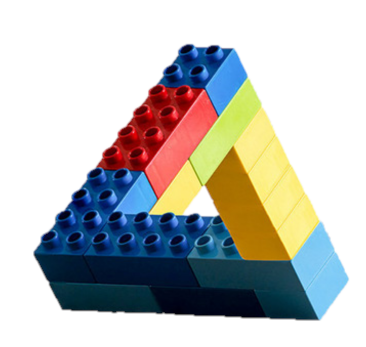
\includegraphics[scale=0.5]{img/penrose-triangle.eps}
 \captionsetup{labelformat=empty}
 \caption{彭罗斯三角形}
 \label{fig:Penrose-triangle}
\end{wrapfigure}

记得在中学数学课上,老师会在黑板上写一个充满字母的式子,然后让同学们化简。有同学会自告奋勇到讲台上拿起粉笔在黑板上推导。合并同类项、因式分解、各种办法都可以用。这个过程就像是变魔术,最后往往得到意想不到的简单结果。当然也有卡住或者绕圈子的时候,老师总是耐心地提示,引导我们找到思路。

这样的经历好像就发生在眼前,一方面,满手的粉笔灰让同学们体会到老师的不易,另一方面,那种推理的神秘强力量让我感到它的强大。我总是希望知道更多的公式,这样就能在化简或者推导时派上用场。

这种推理的神奇之处在于,我们不用特别关心这些公式或者定理在当时场景下的具体含义。就像摆动积木一样,从散落的各种零件,最后搭建起一个有趣玩具。这些公式和定理相互组装到一起,最后引向一个有趣的结果。看到$a^2 + 2ab + b^2$就会把它变换为$(a+b)^2$,就像把两块积木插到一起那样自然,我们不用在推理时强迫自己回想这个公式的几何意义。

\begin{figure}[htbp]
\centering
\begin{tikzpicture}
\draw[fill=gray, draw=black, pattern=north west lines]
  (0, 0) rectangle (4, 4);
\filldraw[fill=white]
  (0, 0) rectangle (1, 1)
  (1, 1) rectangle (4, 4);
\path (0.5, 0.5) node {$a^2$}
      (2.5, 2.5) node {$b^2$}
      (-0.5, 0.5) node {$a$}
      (2.5, 0.5) node {$ab$}
      (4.5, 2.5) node {$b$}
      (0.5, 2.5) node {$ab$};
\path (0, -1) node (l) {}
      (2, -1) node (m) {$a + b$}
      (4, -1) node (r) {};
\draw[->] (m) -- (l);
\draw[->] (m) -- (r);
\end{tikzpicture}
\caption{$(a + b)^2 = a^2 + 2ab + b^2$的几何意义}
\end{figure}

本章中,我们用两个例子说明如何进行编程中的推理。每个例子都首先用直观的方法给出分析和解释,然后再用纯推理的方式给出另一个解法。这就像$(a+b)^2$的情形。一方面我们可以用几何的直观,将其理解为一大一小两个小正方形和两个相等的矩形的面积;另一方面,我们也可以用纯推理一步一步导出同样的结果。

\[
\begin{array}{rcll}
(a + b)^2 & = & (a + b)(a + b) & \text{二次方的定义} \\
          & = & a(a + b) + b(a + b) & \text{乘法分配律} \\
          & = & a^2 + ab + ba + b^2 & \text{再次用分配律} \\
          & = & a^2 + 2ab + b^2 & \text{合并同类项$ab$和$ba$}
\end{array}
\]

\section{叠加——构建的融合}

我们要举的第一个例子是叠加——构建的融合(foldr/build fusion law)。2015年Java在其1.8版本中加入了lambda表达式并且提供了一系列支持函数式编程的工具。但是有人很快发现,尽管一连串地函数调用表达能力很强,简洁优雅,但是性能会下降很多。原因之一就是这些串起来函数调用产生了大量中间结果。这些中间结果往往不是一两个简单的数值,而通常是列表、容器这样规模很大的结构。这些结构被下一个函数消费使用,然后就丢弃了。但是接下来会产生另一个同等规模的结构。这种产生——一次性消费——丢弃——再产生的过程,沿着函数调用链一环一环地重复,造成了很大浪费。

例如\cite{GLPJ-1993},我们想判断一个列表中的每个元素是否都满足某个条件。可以这样定义:

\[
all(p, xs) = and(map(p, xs))
\]

传入$all(prime, [2, 3, 5, 7, 11, 13, 17, 19, ...])$就可以判断是否列表中都是素数。但是这个实现的效率却不高。首先$map(prime, xs)$会产生一个和$xs$同样长度的列表,列表中的每个元素是一个布尔值[True, True, ...],每个布尔值表示对应的元素是不是素数。然后这个布尔值列表传入$and$函数,检查是否存在False。最后$xs$和布尔值列表都被丢弃,而仅仅返回一个布尔值作为最终结果。

下面是另一种定义,它能够避免产生中间的布尔值列表:

\[
\begin{array}{l}
all(p, xs) = h(xs) \\
  \begin{cases}
  h([]) = True \\
  h(x:xs) = p(x) \land h(xs) \\
  \end{cases}
\end{array}
\]

虽然这个实现不产生中间结果,可是和前面的$and(map(p, xs)$比起来,既冗长又不直观。有没有什么办法,鱼和熊掌兼得,即不丧失直观性,又能避免低效的实现呢?我们发现有些变换满足这一要求。例如:

\[
map\ sqrt\  (map\ abs\ xs) = map\ (sqrt \circ abs) xs
\]

先把列表中每个元素取绝对值构成一列新数,然后再把这列数中的每个开方。这和把列表中每个数先取绝对值然后再立即开方后构成一列新数等价。由此我们可以得到一个转换规则:

\be
map\ f\ (map\ g\ xs) = map\ (f \circ g)\ xs
\ee

但是这样的规则太多了,我们无法全部把它们列出。并且在千变万化的程序中,我们无法一眼就看出应该用哪一条规则优化。吉尔(Gill)、朗奇布瑞(Launchbury)、佩顿琼斯(Peyton Jones)在1993年提出了一个方法,他们从列表最本质的构造和叠加操作入手,找到了优化的规律。

\subsection{列表的叠加操作}

我们在第一章就给出过列表的叠加操作,它的定义为:

\[
\begin{array}{l}
foldr\ \oplus\ z\ [] = z \\
foldr\ \oplus\ z\ (x:xs) = x\ \oplus\ (foldr\ \oplus\ z\ xs) \\
\end{array}
\]

展开就是:

\be
foldr\ \oplus\ z\ [x_1, x_2, ..., x_n] = x_1 \oplus (x_2 \oplus (...(x_n \oplus z))...)
\ee

许多列表相关的操作都可以用叠加来定义。我们接下来给出一些典型的例子:

\begin{enumerate}
\item 累加:

\[
sum = foldr\ +\ 0
\]

\item 前面提到的$and$函数,计算一个布尔值列表中的所有元素的逻辑与:

\[
and = foldr\ \land\ True
\]

这是因为:

\[
and\ [x_1, x_2, ..., x_n] = x_1 \land (x_2 \land (...(x_n \land True))...)
\]

\item 在一个列表中查找某一个元素是否存在:

\[
elem\ x\ xs\ = foldr\ (a\ b \mapsto a = x \lor b)\ False\ xs
\]

\item 逐一映射:

\[
\begin{array}{rcl}
map\ f\ xs & = & foldr\ (x\ ys \mapsto f(x) : ys)\ []\ xs \\
           & = & foldr\ ((:) \circ f)\ []\ xs \\
\end{array}
\]

\item 用某一条件过滤列表中的元素:

\[
\begin{array}{rl}
filter\ f\ xs = foldr\ (x\ ys \mapsto
  \begin{cases}
    f(x): & x:ys\ \\
    \text{否则}: & ys
  \end{cases})\ []\ xs \\
\end{array}
\]

\item 两个列表连接:

\[
xs \doubleplus ys = foldr\ (:)\ ys\ xs
\label{eq:binary-concat}
\]

这是因为:

\[
[x_1, x_2, ..., x_n] \doubleplus ys = x_1 : (x_2 : (...(x_n : ys))...)
\]

\item 多个列表连接:

\[
concat\ xss = foldr\ \doubleplus\ []\ xss
\]

\end{enumerate}

叠加操作是如此基本,如果我们能把列表的叠加操作的化简规律找到,就找到了几乎所有列表操作的化简规律。

\subsection{叠加——构建融合律}
现在我们考虑,如果把空列表[](即Nil)和连接操作“:”(即Cons)进行叠加会产生什么结果。

\be
foldr\ (:)\ []\ [x_1, x_2, ..., x_n] = x_1 : (x_2 : (...(x_n : []))...)
\label{eq:foldr-fixed-point}
\ee

这回我们得到了列表本身。你也许想到了上一章介绍的不动点,我们稍后会回到这个话题。换言之,如果我们有一个运算$g$,它能够从一个起始值,例如[],和一个二元组合运算,例如“:”,产生一个列表。我们可以定义这个列表构造过程$build$:

\be
build(g) = g((:), [])
\label{eq:build-definition}
\ee

接着,如果用另一个起始值$z$和二元组合运算$f$,对这一列表进行叠加,其结果就相当于用$z$替换[],用“$f$”替换“(:)”,然后直接调用过程$g$。

\be
\pmb{foldr}(f, z, \pmb{build}(g)) = g(f, z)
\ee

写成无参数括号的形式就是:

\be
\pmb{foldr}\ f\ z\ (\pmb{build}\ g) = g\ f\ z
\label{eq:foldr-build-fusion-law}
\ee

我们称这一结果为\textbf{叠加——构建融合定律}。

在继续深入介绍前,让我们先看一些具体的例子。考虑如何计算从$a$到$b$间的整数和$sum([a, a+1, ..., b-1, b])$。为此我们可以先产生从$a$到$b$之间的所有整数$a, a+1, a+2, ..., b-1, b$,例如使用下面的方法:

\[
range(a, b) =
\begin{cases}
a > b: & [] \\
\text{否则}: & a : range(a+1, b) \\
\end{cases}
\]

这样$range(1, 5)$就产生列表[1, 2, 3, 4, 5]。现在我们只要把这个列表中的元素累加起来就得到答案了:

\[
sum(range(a, b))
\]

接下来关键的一步,我们把$range$中的起始值[]和二元组合运算(:)抽出成为参数:

\[
range'(a, b, \oplus, z) =
  \begin{cases}
  a > b: & z \\
  \text{否则}: & a \oplus range'(a+1, b, \oplus, z) \\
  \end{cases}
\]

我们甚至可以把$range'$的后两个参数克里化:

\[
range'\ a\ b = f\ c \mapsto
  \begin{cases}
  a > b: & c \\
  \text{否则}: & f\ a\ (range' (a+1)\ b\ f\ c) \\
  \end{cases}
\]

这样原来的$range$就可以用$range'$和$build$表示了:

\[
range(a, b) = build(range'(a, b))
\]

写下来我们用融合律化简累加和的计算:

\[
\begin{array}{rcll}
sum(range(a, b)) & = & sum(build(range'(a, b))) & \text{代入} \\
  & = & \pmb{foldr}\ (+)\ 0\ (\pmb{build}\ (range'\ a\ b)) & \text{用叠加表示累加} \\
  & = & range'\ a\ b\ (+)\ 0 & \text{使用融合律} \\
\end{array}
\]

这样就完成了化简,避免产生了中间列表。优化了算法。我们可以看一下最后算法的效果:

\[
range'\ a\ b\ (+)\ 0 =
  \begin{cases}
  a > b: & 0 \\
  \text{否则}: & a + range'(a+1, b, (+), 0) \\
  \end{cases}
\]

\subsection{列表的构建形式}

为了方便使用融合律,我们可以把常见的能够产生新列表操作都写为$build...foldr$的形式。这样当用叠加操作和这种形式的操作组合起来时,$\pmb{foldr}...(\pmb{build}...foldr)$,就可以使用融合律化简。

\begin{enumerate}
\item 首先是最简单的操作——构造空列表:

\[
[] = build\ (f\ z \mapsto z)
\]

我们可以代入$build$的定义(\ref{eq:build-definition})来验证这个定义:

\begin{proof}
\bre
build\ (f\ z \mapsto z) & = & (f\ z \mapsto z)\ (:)\ [] & build\text{的定义} \\
  & = & (:)\ [] \mapsto [] & \beta-\text{规约,参见第二章} \\
  & = & [] & \\
\ere
\end{proof}

\item 接下来是列表的链接(Cons)操作:

\[
x : xs = build\ (f\ z \mapsto f\ x\ (foldr\ f\ z\ xs))
\]

我们来验证一下:

\begin{proof}
\blre
  & build\ (f\ z \mapsto f\ x\ (foldr\ f\ z\ xs)) & \\
= & (f\ z \mapsto f\ x\ (foldr\ f\ z\ xs))\ (:)\ [] & build\text{的定义} \\
= & x : (foldr\ (:)\ []\ xs) & \beta-\text{规约} \\
= & x : xs & \text{由(\ref{eq:foldr-fixed-point}),叠加的不动点} \\
\elre
\end{proof}

\item 然后是列表的连接:

\[
xs \doubleplus ys = build\ (f\ z \mapsto foldr\ f\ (foldr\ f\ z\ ys)\ xs)
\]

\begin{proof}
\blre
  & build\ (f\ z \mapsto foldr\ f\ (foldr\ f\ z\ ys) xs) & \\
= & (f\ z \mapsto foldr\ f\ (foldr\ f\ z\ ys)\ xs)\ (:)\ [] & build \text{的定义} \\
= & foldr\ (:)\ (foldr\ (:)\ []\ ys)\ xs & \beta-\text{规约} \\
= & foldr\ (:)\ ys\ xs & \text{对内层用叠加的不动点} \\
= & xs \doubleplus ys & \text{由(\ref{eq:binary-concat}),列表的连接} \\
\elre
\end{proof}

\end{enumerate}

以下操作我们只列出结果,而把它们的证明作为本小节的练习。

\begin{enumerate}
\setcounter{enumi}{3}
\item 多个列表的连接:
\[
concat\ xss = build\ (f\ z \mapsto foldr\ (xs\ x \mapsto foldr\ f\ x xs)\ xss)
\]

\item 一一映射产生新列表:

\[
map\ f\ xs = build\ (\oplus\ z \mapsto foldr\ (y\ ys \mapsto (f\ y) \oplus ys)\ z\ xs)
\]

\item 过滤元素产生新列表:

\[
filter\ f\ xs = build\ (\oplus\ z \mapsto foldr\ (x\ xs' \mapsto
  \begin{cases}
    f(x): & x \oplus xs' \\
    \text{否则}: & xs' \\
  \end{cases})\ z\ xs) \\
\]

\item 重复不断产生同一元素的(无穷)列表:

\[
repeat\ x = build\ (\oplus\ z \mapsto let\ r = x \oplus r\ in\ r)
\]

\end{enumerate}

\subsection{使用融合律化简}

接下来我们继续使用刚刚打造好的融合律来化简计算。首先是本节开始时$all(p, xs) = and(map(p, xs))$的例子。

\begin{example}
我们把$and$改为叠加形式,把$map$改为构建形式就可以开始化简了。

\bre
all(p, xs) & = & and(map(p, xs)) & \text{原始定义} \\
  & = & foldr\ \land\ True\ map(p, xs) & and\text{的叠加形式} \\
  & = & \pmb{foldr}\ \land\ True\ \pmb{build}\ (\oplus\ z \mapsto & \\
  &   & \quad \quad foldr\ (x\ ys \mapsto p(x) \oplus ys)\ z\ xs) & map\text{的构建形式} \\
  & = & (\oplus\ z \mapsto foldr\ (x\ ys \mapsto p(x) \oplus ys)\ z\ xs)\ \land\ True & \text{融合律} \\
  & = & foldr\ (x\ ys \mapsto p(x) \land ys)\ True\ xs & \beta-\text{规约} \\
\ere

如果使用第一章介绍过的$first$函数,还可以进一步化简为:

\[
all\ p = foldr\ (\land) \circ (first\ p)\ True
\]

\end{example}

\begin{example}
我们举的第二个例子是把若干词语添加上空格,然后连接成句子。这样的文字处理过程通常叫做$join$,简单起见,我们在句子最后也添上一个空格。一个典型的定义如下:

\[
join(ws) = concat(map(w \mapsto w \doubleplus ['\ '], ws))
\]

这个定义简单直观,它先用逐一映射,在每个单词的末尾添加空格,得到一个新的单词列表,然后再把这个列表连接成一个字符串。但是这个定义的性能不佳。首先在单词末尾添加空格就是一个昂贵的计算,需要移动到每个单词的末尾,然后使用字符串连接操作。其次有多少单词,逐一映射就会产生一个同样数量的单词列表。最后这些中间结果都被丢弃了。我们接下来用融合律优化这一计算。

\[ \begin{array}{rl}
  & join(ws) \\
  & \{\text{定义} \} \\
= & concat(map(w \mapsto w \doubleplus ['\ '], ws)) \\

  & \{\text{把$concat$写为构建形式}\} \\
= & build\ (f\ z \mapsto \\
  & \quad foldr\ (x\ y \mapsto foldr\ f\ y\ x)\ z\ map(w \mapsto w \doubleplus ['\ '], ws)) \\

  & \{\text{把$map$写为构建形式}\} \\
= & build\ (f\ z \mapsto \\
  & \quad \pmb{foldr}\ (x\ y \mapsto foldr\ f\ y\ x)\ z\ (\pmb{build}\ (f'\ z' \mapsto \\
  & \quad \quad foldr\ (w\ b \mapsto f'\ (w \mapsto w \doubleplus ['\ '])\ b)\ z'\ ws))) \\

  & \{\text{融合律}\} \\
= & build\ (f\ z \mapsto \\
  & \quad foldr\ (w\ b \mapsto (x\ y \mapsto foldr\ f\ y\ x)\ (w \doubleplus ['\ '])\ b)\ z\ ws) \\

  & \{\beta-\text{规约}x, y\} \\
= & build\ (f\ z \mapsto \\
  & \quad foldr\ (w\ b \mapsto foldr\ f\ b\ (w \doubleplus ['\ ']))\ z\ ws) \\

  & \{\text{把$\doubleplus$写为构建形式}\} \\
= & build\ (f\ z \mapsto \\
  & \quad foldr\ (w\ b \mapsto \\
  & \quad \quad \pmb{foldr}\ f\ b\ (\pmb{build}\ (f'\ z' \mapsto \\
  & \quad \quad \quad foldr\ f'\ (foldr\ f'\ z'\ ['\ '])\ w)))\ z\ ws) \\

  & \{\text{融合律}\} \\
= & build\ (f\ z \mapsto \\
  & \quad foldr\ (w\ b \mapsto \\
  & \quad \quad foldr\ (foldr\ f\ b\ ['\ '])\ w)\ z\ ws) \\

  & \{\text{据$build$的定义,将$(:)$和$[]$代入}\} \\
= & foldr\ (w\ b \mapsto foldr\ (:)\ \pmb{(foldr\ (:)\ b\ ['\ '])}\ w)\ []\ ws \\

  & \{\text{对黑体字部分求值}\} \\
= & foldr\ (w\ b \mapsto foldr\ (:)\ ('\ ' : b)\ w)\ []\ ws \\
\end{array} \]

因此最后化简的结果为:

\[
join(ws) = foldr\ (w\ b \mapsto foldr\ (:)\ ('\ ' : b)\ w)\ []\ ws
\]

我们还可以据此把叠加操作展开,得到一个可读性较好的优化定义:

\[
\begin{array}{l}
\begin{cases}
join\ [] = [] \\
join\ (w:ws) = h\ w \\
\end{cases} \\
\text{其中}: \begin{cases}
             h\ [] = '\ ' : join\ ws \\
             h\ (x:xs) = x : h\ xs \\
             \end{cases} \\
\end{array}
\]

由于$concat \circ map(f)$十分常见,很多编程环境的标准库已经提供了这样的优化实现。例如Haskell中的\texttt{concatMap},Java和Scala中的\texttt{flatMap}。
\end{example}

第二个例子虽然展示了融合律的强大,但是也暴露出了一个问题。推导过程机械繁琐、容易出错。这恰恰是机器,而非人类擅长的事情。有些编程环境,例如Haskell已经把融合律实现在编译器内部\cite{GLPJ-1993}。这样只要我们把列表的常见操作用构建、叠加形式定义好,机器就可以替代我们利用融合律进行上述化简,从而得到优化的程序,避免中间结果和多余的递归\footnote{例如Haskell标准库已经用构建、叠加形式实现了大多数列表操作。}。随着时间的推移,更多的编译器会逐渐支持这一优化工具。

\subsection{类型限制}

每当我们打造出抽象的工具,就要思考它的适用范围,了解它什么情况下会失效。对于融合律也是如此。考虑下面的矛盾结果:

\blre
  & \pmb{foldr}\ f\ z\ (\pmb{build}\ (c\ n \mapsto [0])) & \\
= & (c\ n \mapsto [0])\ f\ z & \text{融合律} \\
= & [0] & \beta-\text{规约} \\
\elre

另一方面:

\blre
  & foldr\ f\ z\ (build\ (c\ n \mapsto [0])) & \\
= & foldr\ f\ z\ ((c\ n \mapsto [0])\ (:)\ []) & build\text{的定义} \\
= & foldr\ f\ z\ [0] & \beta-\text{规约} \\
= & f(0, z) & \text{叠加展开} \\
\elre

显然$f(0, z)$不等于$[0]$,它们两个的类型都甚至不同\footnote{除非极特殊情况$f = (:), z = []$。}。造成这一矛盾结果的原因是$(c\ n \mapsto [0])$不是一个真正用$c$和$n$构造结果的函数。为此我们需要对融合律$foldr\ f\ z\ (build\ g) = g\ f\ z$中$g$的类型做出限制。它的第一个参数既可以接受$c$,也可以接受$f$,换言之,它接受一个多态的二元运算$\forall A. \forall B.\ A \times B \to B$;同理它的第二个参数也是一个多态类型$B$的起始值,并产生一个类型为$B$的结果。我们把二元运算写为克里化的形式就得到:

\[
g : \forall A. (\forall B. (A \to B \to B) \to B \to B)
\]

容易看出,上面反例中的类型是:$\forall A. (\forall B. (A \to B \to B) \to B \to [Int])$。不满足我们的类型限制。与此对应,构建函数$build$的类型为:

\[
build : \forall A. (\forall B. (A \to B \to B) \to B \to B) \to \mathbf{List}\ A
\]

由于里面有两个多态的类型$A$和$B$,因此它被称为二阶多态函数(rank-2 type polymorphic)。

\subsection{用范畴论推导融合律}

叠加——构建融合律可以用范畴理论推导出来并进行扩展。一旦把范畴论作为理论工具,人们就发现叠加——构建融合仅仅是众多种融合规则中的一个。现在这些规则统一被称为“短路融合”(shortcut fusion)。它们在编译器优化,程序库优化中发挥了重要的作用。我们无法在这一章中对它们做全面的介绍。读者可以参考\cite{Hinze-Harper-James-2010}深入了解短路融合的理论和实践方法。

在上一章中,我们介绍了F-代数,特别是初始代数和向下态射。由于初始代数是起始对象,所以它到任何其他代数都有唯一的箭头。如下图所示:

\begin{center}
\begin{tikzpicture}
  \matrix (m) [matrix of math nodes,
               row sep=3em, column sep=3em, minimum width=2em]{
    \mathbf{F} I  & I \\
    \mathbf{F} A  & A \\};
  \path[-stealth]
    (m-1-1) edge node [above] {$i$} (m-1-2)
    (m-1-1) edge node [left] {$\mathbf{F} \lbb a \rbb$} (m-2-1)
    (m-1-2) edge node [right] {$\lbb a \rbb$}  (m-2-2)
    (m-2-1) edge node [below] {$a$} (m-2-2);
\end{tikzpicture}
\end{center}

从初始代数$(I, i)$到另一代数$(A, a)$的箭头可以通过向下态射$\lbb a \rbb$来表示。如果还存在一个不同的F-代数$(B, b)$对象,并且有从$A$到$B$的箭头$A \arrowto{h} B$,就可以在上面的范畴图下方把$(B, b)$也画出:

\begin{center}
\begin{tikzpicture}
  \matrix (m) [matrix of math nodes,
               row sep=3em, column sep=3em, minimum width=2em]{
    \mathbf{F} I & I \\
    \mathbf{F} A & A \\
    \mathbf{F} B & B \\};
  \path[-stealth]
    (m-1-1) edge node [above] {$i$} (m-1-2)
    (m-1-1) edge node [left] {$\mathbf{F} \lbb a \rbb$} (m-2-1)
    (m-1-2) edge node [right] {$\lbb a \rbb$}  (m-2-2)
    (m-2-1) edge node [below] {$a$} (m-2-2)
    (m-3-1) edge node [below] {$b$} (m-3-2)
    (m-2-1) edge node [left] {$\mathbf{F}(h)$} (m-3-1)
    (m-2-2) edge node [right] {$h$} (m-3-2);
\end{tikzpicture}
\end{center}

但由于$(I, i)$是起始对象,所以它到$(B, b)$也必然存在唯一的箭头。由此可知,必然存在从$I$到$B$的箭头,可以用向下态射$\lbb b \rbb$表示出来。如下图:

\begin{center}
\begin{tikzpicture}
  \matrix (m) [matrix of math nodes,
               row sep=3em, column sep=3em, minimum width=2em]{
    \mathbf{F} I & I & \\
    \mathbf{F} A & A & \lbb b \rbb \\
    \mathbf{F} B & B & \\};
  \path[-stealth]
    (m-1-1) edge node [above] {$i$} (m-1-2)
    (m-1-1) edge node [left] {$\mathbf{F} \lbb a \rbb$} (m-2-1)
    (m-1-2) edge node [right] {$\lbb a \rbb$}  (m-2-2)
    (m-2-1) edge node [below] {$a$} (m-2-2)
    (m-3-1) edge node [below] {$b$} (m-3-2)
    (m-2-1) edge node [left] {$\mathbf{F}(h)$} (m-3-1)
    (m-2-2) edge node [right] {$h$} (m-3-2);
  \draw[-stealth]
    (m-1-2) .. controls (m-2-3) .. (m-3-2);
\end{tikzpicture}
\end{center}

从这个范畴图可以看出,如果存在$h$,则下面那个小正方形可交换。这等价于说从$I$经由$A$到$B$相当于从$I$直接到$B$。这就是初始代数的融合律。记为:

\be
\begin{array}{rcl}
A \arrowto{h} B \Rightarrow h \circ \lbb a \rbb = \lbb b \rbb
& \iff &
h \circ a = b \circ \mathbf{F}(h) \\
\end{array}
\ee

初始代数的融合律意味这什么呢?在上一章中,我们发现向下态射可以将非递归的计算,转换成在递归结构上的叠加计算。例如,当函子$\mathbf{F}$是$\mathbf{ListF}A$(其中$A$是给定的对象)时,箭头$a = f + z$(加号表示余积),而初始箭头$i = (:) + []$,向下态射$\lbb a \rbb = foldr(f, z)$。如果记$b = c + n$,则融合律可以写成:

\[
h \circ foldr(f, z) = foldr(c, n)
\]

它说明叠加之后再进行变换可以化简为单一的叠加。1995年,高野秋彦和梅耶(Meijer)进一步将向下态射$\lbb a \rbb$抽象成从$a$构造某种代数结构$g\ a$,这样融合律就可以推广为\cite{Takano-Meijer-1995}:

\be
A \arrowto{h} B \quad \Rightarrow \quad h \circ g\ a = g\ b
\ee

这一推广的融合律被称为“酸雨定律”\footnote{由于融合律能够消除不必要的中间结果,所以最早被称为“砍伐定律”(deforestation),所以推广的融合律被幽默地称为酸雨定律(acid rain law)。}。另一方面,由于存在从初始代数$I$到$A$的箭头:$I \arrowto{\lbb a \rbb} A$,所以将$\lbb a \rbb$代入酸雨定律左侧的$h$,并且用$i$替换酸雨定律中的$a$,用$a$替换酸雨定律中的$b$,我们有:

\be
I \arrowto{\lbb a \rbb} A \quad \Rightarrow \quad \lbb a \rbb \circ g\ i = g\ a
\ee

具体到列表的例子,把$\lbb a \rbb$代换为$foldr(f, z)$;把初始代数$i$代换为列表的初始代数$(:) + []$;定义$build(g) = g\ (:)\ []$,并代入酸雨定律左侧,就得到了列表的叠加——构建融合律:

\blre
& \lbb a \rbb \circ g\ i = g\ a & \text{酸雨定律} \\

\Rightarrow &
foldr\ f\ z\ (g\ i) = g\ a & \text{列表的向下态射是叠加} \\

\Rightarrow &
foldr\ f\ z\ (g\ (:)\ []) = g\ a & \text{列表的初始代数$i$是$(:), []$} \\

\Rightarrow &
foldr\ f\ z\ (g\ (:)\ []) = g\ f\ z & \text{用$f, z$替换$a$} \\

\Rightarrow &
\pmb{foldr}\ f\ z\ (\pmb{build}\ g) = g\ f\ z & \text{反向用$build$的定义} \\
\elre

这样我们就用范畴论证明了叠加——构建融合律\cite{Hinze-Harper-James-2010}。

\begin{Exercise}
\Question{验证从左侧叠加也可以表示为$foldr$:
\[
foldl\ f\ z\ xs = foldr\ (b\ g\ a \mapsto g\ (f\ a\ b))\ id\ xs\ z
\]}
\Question{证明以下列表的构建——叠加形式:
\[
\begin{array}{l}
concat\ xss = build\ (f\ z \mapsto foldr\ (xs\ x \mapsto foldr\ f\ x xs)\ xss) \\
map\ f\ xs = build\ (\oplus\ z \mapsto foldr\ (y\ ys \mapsto (f\ y) \oplus ys)\ z\ xs) \\
filter\ f\ xs = build\ (\oplus\ z \mapsto foldr\ (x\ xs' \mapsto
  \begin{cases}
     f(x): & x \oplus xs' \\
    \text{否则}: & xs' \\
  \end{cases})\ z\ xs) \\
repeat\ x = build\ (\oplus\ z \mapsto let\ r = x \oplus r\ in\ r) \\
\end{array}
\]
}
\Question{利用融合律化简快速排序算法:
\[
\begin{cases}
qsort\ [] = [] \\
qsort\ (x:xs) = qsort\ [a | a \in xs, a \leq x] \doubleplus [x] \doubleplus qsort\ [a | a \in xs, x < a] \\
\end{cases}\]
提示:将ZF表达式\footnote{全称为“策梅罗——弗兰克尔表达式”。指集合论中$\{f(x) | x \in X, p(x), q(x), ...\}$这样的集合构建表达式。我们在下一章介绍无穷和集合论时会再次遇到它。}转换为$filter$。}
\Question{利用范畴论验证融合律的类型限制。提示:考虑向下态射的类型。}
\end{Exercise}

\section{巧算100}

我们举的第二个例子来自伯德的《函数式算法珠玑》中的第6章\cite{Bird-2010}。高德纳在《计算机程序设计的艺术》卷4中给出了一道练习题\cite{Knuth-TAOCP-2006}:把1到9这九个数字写成一行:1 2 3 4 5 6 7 8 9。只允许在这些数字之间添上加号和乘号,不许用括弧。如何使得最后的得数恰好是100?

例如:

\[
12 + 34 + 5 \times 6 + 7 + 8 + 9 = 100
\]

这看起来像是一道小学生的数学竞赛题目。如果要求找到所有可能的解法,就是一道编程趣题。最简单直接的方法,就是利用计算机进行穷举,每两个数字间一共有三种选择:1)什么都不插入;2)插入加号;3)插入乘号。由于九个数字间一共有8个空,所以共有$3^8 = 6561$种方法。我们只要让计算机逐一检查这6561种方案,看看哪些最终得数是100就可以了。

\subsection{穷举法}

为此,我们先把一个由数字、加法、乘法组成的式子定义出来。考虑刚才的算式:

\[
12 + 34 + 5 \times 6 + 7 + 8 + 9
\]

由于先乘除后加减,我们可以把它看作由加号分割的若干子算式。所以上述算式的等价于:

\[
sum [12, 34, 5 \times 6, 7, 8, 9]
\]

这样我们定义一个算式是由加号分割的若干子算式。即$expr = [t_1, t_2, ..., t_n]$:

\lstset{frame = none}
\begin{lstlisting}
type Expr = [Term]
\end{lstlisting}

具体到每个子算式,我们可以把它看作由乘号分割的若干因子,例如$5 \times 6 = product [5, 6]$。如果是单一的数,例如$34$,我们仍然可以把它看作$34 = product [34]$。这样我们就可以定义由因子组成的子算式。即$term = [f_1, f_2, ..., f_m]$:

\begin{lstlisting}
type Term = [Factor]
\end{lstlisting}

最终,每个因子都可以看作若干数字组成的整数,例如由两个数字组成的34,或仅有一个数字的5。也就是说$factor = [d_1, d_2, ..., d_k]$:

\begin{lstlisting}
type Factor = [Int]
\end{lstlisting}

从若干数字求得整数是一个叠加的过程,例如$[1, 2, 3] \Rightarrow (((1 \times 10) + 2) \times 10) + 3$。我们可以将其定义为一个函数:

\[
dec = foldl\ (n\ d \mapsto n \times 10 + d)\ 0
\]

穷举法的思路是针对每一个可能的表达式,计算并检查它是否得100。为此,我们需要定义一个函数,求出一个表达式的值。根据表达式的定义,我们需要递归地求出每个子表达式(term)的值,然后将其累加起来;为了求每个子表达式的值,需要递归地求出每个因子的值,然后再累乘起来;为了求每个因子的值,需要对每个因子使用$dec$函数。

\[
eval = sum \circ map\ (product \circ (map\ dec))
\]

明显这一定义可以用上一节介绍的融合律进行优化,我们把具体的推导过程留作练习。最终的优化结果如下:

\[
eval = foldr\ (t\ ts \mapsto (foldr\ ((\times) \circ fork(dec, id))\ 1\ t) + ts)\ 0
\]

从这一结果可以写出一个可读性与性能都更好的定义:

\[
\begin{cases}
eval\ [] = 0 \\
eval (t:ts) = product\ (map\ dec\ t) + eval(ts) \\
\end{cases}
\]

根据这一定义,如果表达式为空,则其值为0;否则我们取出第一个子表达式,将其中的每个因子求出并乘到一起。然后再加上剩余子表达式的求值结果。这样在使用穷举法时,对每个可能的表达式,我们都用$eval$求值。留下所有等于100的表达式。即:

\[
filter\ (e \mapsto eval(e) == 100)\ es
\]

其中$es$是所有从1到9能够组成的表达式的集合。如何产生这个集合呢?我们从空集合开始,然后每次从1到9中取出一个数字,看看能扩展出哪些合法的表达式。首先,从空集合和唯一的数字$d$只能构造出一个表达式:$[[[d]]]$。最内层是由数字$d$构成的唯一因子$fact = [d]$;然后是由这个因子构成的子表达式$term = [fact] = [[d]]$,这个唯一的子表达式构成的完整表达式是$[term] = [[fact]] = [[[d]]]$。我们可以把这一构造过程定义为:

\[
expr(d) = [[[d]]]
\]

接下来,考虑一般情形。我们的策略是从右侧开始,不断取出数字9, 8, 7, ...来扩展表达式。假设我们已经用数字构造了一个表达式集合$[e_1, e_2, ..., e_n]$,此时如果取出下一个数字$d$,如何扩展出所有的合法表达式呢?我们在本节的开头说过,每两个数字间一共由三种选择:1)什么都不插入;2)插入加号;3)插入乘号。我们来看看对于表达式集合中的任意$e_i$这三种选择的含义分别是什么。将$e_i$展开表示成若干子表达式的和$e_i = t_1 + t_2 + ...$,其中第一个子表达式$t_1$表示为若干因子的积$t_1 = f_1 \times f_2 \times ...$。

\begin{enumerate}
\item 什么都不插入意味着将数字$d$直接添加到$e_i$的第一个子表达式中的第一个因子的前面。这样由$d:f_1$组成一个新的因子。例如$e_i$是表达式$8 + 9$,数字$d$是7,将7写在$8+9$的前面而什么符号都不插入,这样就得到新表达式$78 + 9$;
\item 插入乘号意味着用数字$d$构成一个因子$[d]$,然后将它添加到$e_i$中第一个字表达式的前面。这样由$[d]:t_1$组成一个新的子表达式。具体到$8 + 9$这个例子,我们把7写在它的前面,然后在7和8之间插入一个乘号,这样就得到新表达式$7 \times 8 + 9$;
\item 插入加号意味着用数字$d$构成一个子表达式$[[d]]$,然后将将它添加到$e_i$的最前面,组成新的表达式$[[d]]:e_i$。具体到$8 + 9$这个例子,我们把7写在它的前面,然后在7和8之间插入一个加号,这样就得到新表达式$7 + 8 + 9$;
\end{enumerate}

把这三种情形转换为定义就得到了下面的函数:

\lstset{frame = none}
\begin{lstlisting}
add d ((ds:fs):ts) = [((d:ds):fs):ts,
                      ([d]:ds:fs):ts,
                      [[d]]:(ds:fs):ts]
\end{lstlisting}

其中表达式$e_i$被写成了$(ds:fs):ts$的形式,$e_i$中的第一个子表达式是$ds:fs$,第一个子表达式中的第一个因子是$ds$。这样,从每个已有的表达式,我们都可以扩展出3个新表达式。而对于表达式列表$[e_1, e_2, ..., e_n]$,只要分别对每个表达式扩展,然后将结果连接到一起就可以了。这恰恰就是上一节我们介绍过的$concatMap$:

\[
\begin{cases}
extend\ d\ [] = [expr(d)] \\
extend\ d\ es = concatMap\ (add\ d)\ es
\end{cases}
\]

这样我们就得到了穷举法的完整定义:

\be
filter\ (e \mapsto eval(e) == 100)\ (foldr\ extend\ [1..9])
\label{eq:puzzle100-basic}
\ee

\subsection{改进}

我们能继续改进这个穷举法么?观察用1到9这些数字从右向左穷举表达式的过程。首先我们写下数字9,在添加数字8时,可能产生3个表达式,分别是:89,$8 \times 9 = 72$,和8 + 9 = 17。接下来添加7,表达式789显然大于100,可以立即丢弃。并且我们确信任何在789左侧扩展出的新表达式也都不可能等于100,因此也可以丢弃。这样就避免了无谓的计算。同样$7 \times 89$也大于100,可以丢弃并停止向左扩展。只有7+89是可能的候选表达式。接下来我们扩展出$78 \times 9$,由于它大于100,因此被丢弃并停止扩展……

通过这一过程,我们发现,可以一边扩展表达式,一边计算当前表达式的值。只要超过100就丢弃并停止从这一候选表达式向左继续扩展。整个过程就像一棵不断生长的树,只要树枝代表的表达式超过100,就砍掉树枝,停止这一分支的生长。

\begin{figure}[htbp]
\centering
\begin{tikzpicture}
\path (0, 0)  node[rectangle, draw] (9) {9}
      (-4, 1) node[rectangle, draw] (89) {89}
      (0, 1)  node[rectangle, draw] (8x9) {$8 \times 9$}
      (4, 1)  node[rectangle, draw] (8+9) {$8 + 9$}
      (-5.5, 2) node[rectangle, draw] (789) {\sout{789}}
      (-4, 2) node[rectangle, draw] (7x89) {\sout{$7 \times 89$}}
      (-2.5, 2) node[rectangle, draw] (7+89) {$7 + 89$}
      (-2, 3) node[rectangle, draw] (78x9) {\sout{$78 \times 9$}}
      (-0.5, 3)  node[rectangle, draw] (7x8x9) {\sout{$7 \times 8 \times 9$}}
      (1.5, 3)  node[rectangle, draw] (7+8x9) {$7 + 8 \times 9$}
      (2, 2)  node[rectangle, draw] (78+9) {$78 + 9$}
      (3.5, 2)  node[rectangle, draw] (7x8+9) {$7 \times 8 + 9$}
      (5.5, 2)  node[rectangle, draw] (7+8+9) {$7 + 8 + 9$};
\draw[->] (9) edge (89)
          (9) edge (8x9)
          (9) edge (8+9)
          (89) edge (789)
          (89) edge (7x89)
          (89) edge (7+89)
          (8x9) edge (78x9)
          (8x9) edge (7x8x9)
          (8x9) edge (7+8x9)
          (8+9) edge (78+9)
          (8+9) edge (7x8+9)
          (8+9) edge (7+8+9);
\end{tikzpicture}
\caption{穷举表达式的过程类似一棵生长的树}
\end{figure}

为了能够一边扩展表达式,一边快速计算当前表达式的值,我们可以将表达式的值分离成三个部分:第一个子表达式中的第一个因子的值$f$,除去$f$外剩余因子的乘积$v_{fs}$,以及除去第一个子表达式外,剩余所有子表达式的和$v_{ts}$。有了这三个部分,我们就可以计算出整个表达式的值$f \times v_{fs} + v_{ts}$。

此时,如果继续向左扩展一个数字$d$,对应三种选择,表达式及其值的更新分别如下:

\begin{enumerate}
\item 不插入任何符号,将$d$添加到第一个因子前作为最高位数字。表达式的值等于:$(d \times 10^{n+1} + f) \times v_{fs} + v_{ts}$,其中$n$是因子$f$的位数。因此值的三个部分更新为:$f' = d \times 10^{n+1} + f$,$v_{fs}$和$v_{ts}$保持不变。
\item 插入乘号,将$d$作为第一个子表达式中的第一个因子。表达式的值等于:$d \times f \times v_{fs} + v_{ts}$。因此值的三个部分更新为:$f' = d, v_{fs'} = f \times v_{fs}$,$v_{ts}$不变。
\item 插入加号,将$d$作为新的第一个子表达式。表达式的值等于:$d + f \times v_{fs} $。因此值的三个部分更新为:$f' = d, v_{fs'} = 1, v_{ts'} = f \times v_{fs} + v_{ts}$。
\end{enumerate}

为了方便第一条中$10^{n+1}$的计算,我们可以把指数也记录下来作为表达式值的第四个部分。这样表达式的值就可以表示为一个四元组$(e, f, v_{fs}, v_{ts})$。从四元组计算表达式值的定义为:

\be
value(e, f, v_{fs}, v_{ts}) = f \times v_{fs} + v_{ts}
\ee

这样在扩展表达式时,我们可以一边扩展,一边更新四元组,并将结果成对放在一起:

\be
\begin{array}{rrl}
add & d\ (((ds:fs):ts), & (e, f, v_{fs}, v_{ts})) = \\
&  [(((d:ds):fs):ts, & (10 \times e, d \times e + f, v_{fs}, v_{ts})), \\
&   (([d]:ds:fs):ts, & (10, d, f \times v_{fs}, v_{ts})), \\
&   ([[d]]:(ds:fs):ts, & (10, d, 1, f \times v_{fs} + v_{ts}))] \\
\end{array}
\ee

对于每一对表达式和四元组,我们利用$value$函数,将四元组的值求出,如果大于100就立即丢弃,停止对其继续扩展。然后将候选表达式和四元组对连接成一个列表。根据这一思路,我们将之前定义的$extend$重新定义为:

\be
\begin{cases}
expand\ d\ [] = [(expr(d), (10, d, 1, 0))] \\
expand\ d\ evs = concatMap\ ((filter\ ((\leq 100) \circ value \circ snd)) \circ (add\ d))\ evs\\
\end{cases}
\ee

现在我们可以对$expand$进行叠加,从1到9扩展出所有小于等于100的候选表达式和四元组。最后我们计算四元组的值,然后选出所有恰好等于100的表达式。

\be
map\ fst \circ filter\ ((=100) \circ value \circ snd)\ (foldr\ expand\ []\ [1, 2, ..., 9])
\ee

在本章附录中,我们给出了根据这一定义编写的程序。下面列出了等于100的所有7个表达式:

\[
\begin{array}{rl}
1: & 1 \times 2 \times 3 + 4 + 5 + 6 + 7 + 8 \times 9 \\
2: & 1 + 2 + 3 + 4 + 5 + 6 + 7 + 8 \times 9 \\
3: & 1 \times 2 \times 3 \times 4 + 5 + 6 + 7 \times 8 + 9 \\
4: & 12 + 3 \times 4 + 5 + 6 + 7 \times 8 + 9 \\
5: & 1 + 2 \times 3 + 4 + 5 + 67 + 8 + 9 \\
6: & 1 \times 2 + 34 + 5 + 6 \times 7 + 8 + 9 \\
7: & 12 + 34 + 5 \times 6 + 7 + 8 + 9 \\
\end{array}
\]

\begin{Exercise}
\Question{利用融合律化简表达式求值的定义$eval = sum \circ map\ (product \circ (map\ dec))$。}
\Question{如何从左侧扩展出所有的表达式?}
\Question{下面定义可以将表达式翻译为字符串:
\[
str = (join\ ``+'') \circ (map\ ((join\ ``*'') \circ (map\ (show \circ dec))))
\]
其中$show$可以将数字转换为字符串。函数$join(c, s)$将一组字符串$s$用$c$连接起来,例如$join(``,'', [``abc'', ``def'']) = ``abc,def''$。利用融合律化简$str$的定义。
}
\end{Exercise}

\section{小节和扩展阅读}

程序推导是数学推导的一种特殊情况。通过这一手段,我们可以从直观的、未经化简或优化的定义出发,利用一套形式化的方法和定理,一步一步进行变换。从而最终得到更加简洁的、优化的结果。伯德在他的《函数式算法设计珠玑》\cite{Bird-2010}中给出了大量的例子,甚至推导出了字符串匹配的博耶尔——摩尔算法和KMP算法。

程序推导的正确性根植于数学。为此需要一套完整的理论,能够将计算机程序形式化、数学化。而不是仅仅依赖于人的直觉。抽象代数和范畴理论正是帮助我们对计算机编程进行形式化的强大工具。叠加——构建融合律就是这样的一个典型的例子。在1993年的论文\cite{GLPJ-1993}中,人们发现了系统化简程序的一个工具。随着范畴理论的引入,一系列融合律通过代数和余代数被发展出来\cite{Hinze-Harper-James-2010}。

\section{附录代码}

Haskell中的\texttt{build}和\texttt{concatMap}定义:

\lstset{frame=single}
\begin{lstlisting}
build :: forall a. (forall b. (a -> b -> b) -> b -> b) -> [a]
build g = g (:) []

concatMap f xs = build (\c n -> foldr (\x b -> foldr c b (f x)) n xs)
\end{lstlisting}

用穷举法巧算100的基本定义:
\begin{lstlisting}
type Expr = [Term]     -- | T1 + T2 + ... Tn
type Term = [Factor]   -- | F1 * F2 * ... Fm
type Factor = [Int]    -- | d1d2...dk

dec :: Factor -> Int
dec = foldl (\n d -> n * 10 + d) 0

expr d = [[[d]]]  -- | single digit expr

eval [] = 0
eval (t:ts) = product (map dec t) + eval ts

extend :: Int -> [Expr] -> [Expr]
extend d [] = [expr d]
extend d es = concatMap (add d) es where
  add :: Int -> Expr -> [Expr]
  add d ((ds:fs):ts) = [((d:ds):fs):ts,
                        ([d]:ds:fs):ts,
                        [[d]]:(ds:fs):ts]

sol = filter ((==100) . eval) . foldr extend []
\end{lstlisting}

用改进的穷举法解决巧算100问题:
\begin{lstlisting}
value (_, f, fs, ts) = f * fs + ts

expand d [] = [(expr d, (10, d, 1, 0))]
expand d evs = concatMap ((filter ((<= 100) . value . snd)) . (add d)) evs where
  add d (((ds:fs):ts), (e, f, vfs, vts)) =
    [(((d:ds):fs):ts, (10 * e, d * e + f, vfs, vts)),
     (([d]:ds:fs):ts, (10, d, f * vfs, vts)),
     ([[d]]:(ds:fs):ts, (10, d, 1, f * vfs + vts))]

sol = map fst . filter ((==100) . value . snd) . foldr expand []
\end{lstlisting}

\ifx\wholebook\relax \else
\begin{thebibliography}{99}

\bibitem{GLPJ-1993}
Andrew Gill, John Launchbury, Simon L. Peyton Jones. ``A Short Cut to Deforestation''. Functional programming languages and computer architecture. pp. 223-232. 1993.

\bibitem{Bird-2010}
Richard Bird. ``Pearls of Functional Algorithm Design''. Cambridge University Press; 1 edition November 1, 2010. ISBN: 978-0521513388.

\bibitem{Hinze-Harper-James-2010}
Ralf Hinze, Thomas Harper, Daniel W. H. James. ``Theory and Practice of Fusion''. 2010, 22nd international symposium of IFL (Implementation and application of functional languages). pp.19-37.

\bibitem{Takano-Meijer-1995}
Akihiko Takano, Erik Meijer. ``Shortcut Deforestation in Calculational Form''. Functional programming languages and computer architecture. pp. 306-313. 1995.

\end{thebibliography}

\expandafter\enddocument
%\end{document}

\fi
